\usepackage{graphicx}
\graphicspath{ {./images/} }
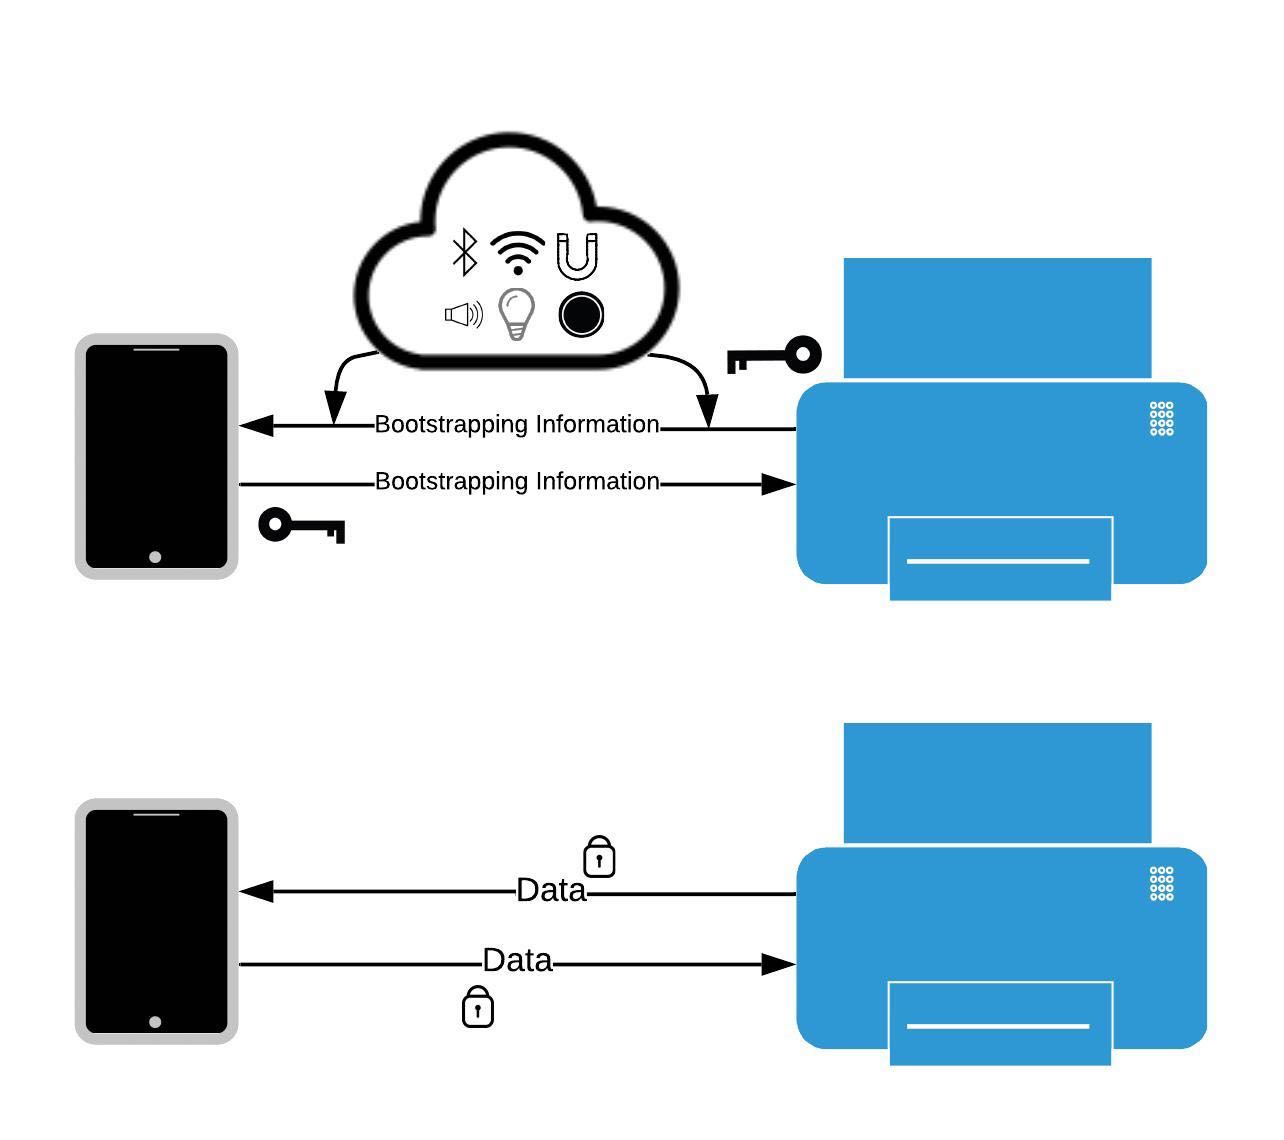
\includegraphics[scale=0.15]{pic}
\section{Bootstrapping Taxonomy}

Out-of-band (OOB) channels are auxiliary to the main frequency of communication and are used as a means to bolster security.
OOB channels are characterized by the uncommon or unused frequencies that the protocols use to communicate or share any cryptographic information.
This section identifies techniques that can be used in the design of onboarding protocols highlighting the security properties and vulnerabilities for each of them. 

\subsection{Bluetooth Low Energy (BLE)}
\subsubsection{Device Provision Protocol (DPP)}
Seamless operations in a smart office involves communications among devices which are separated by small distances.
The functioning of DPP ~\cite{wifialliance} involves two devices: a configurator which broadcasts intent and an enrollee that responds to a broadcast when within the range.
After a response to the broadcast, the devices move to an auxiliary channel via BLE and exchange cryptographic information.
One of the main vulnerabilities of using BLE pairing is that it broadcasts messages openly to any device within range alerting attackers.
BLE itself does not have a proof of possession of the bootstrapping keys in the auxiliary channel.
Any device within range can possibly eavesdrop on both device and obtain the bootstrapping keys.


%As a means for device onboarding, BLE is a viable alternative to Wifi in scenarios that do not require long range communication - not unlike an office. BLE lets a user send out a broadcast that states their intent to bootstrap with another device. The DPP requires two devices: a configurator that broadcasts intent and an enrollee within range that responds to a broadcast. When an enrollee does respond to a broadcast, the devices move to an auxiliary channel via BLE and exchange cryptographic information. One of the primary DPP characteristics is that the configurator sends out a request packet on the auxiliary channel and the enrollee must send back that same auxiliary channel request information to successfully onboard. One of the main vulnerabilities of using BLE pairing is its that broadcasts openly to any device within range. By broadcasting openly, the devices make themselves susceptible to Man in The Middle (MiTM) attacks. BLE itself does not have a proof of possession of the bootstrapping keys in the auxiliary channel. Any device within range can possibly eavesdrop on both device and obtain the bootstrapping keys.


\subsection{Buttons}
\subsubsection{Button Enabled Device Association (BEDA)}
The BEDA protocol ~\cite{soriente2007beda} is reliant on physical buttons on two devices.
These buttons are integral to the protocol because it uses the duration of a pressed button which is used to generate a shared secret.
However, this method presents a few vulnerabilities to replay attacks because hashes are not encrypted when they are sent out which lets an attacker pose as the sender by sending the hash to the original receiving device.



\subsection{Magnetometer Pairing}
Magnetometer pairing is a technique of bootstrapping designed for smartphones by making use of their magnetometers and a WiFi connection. The process is started by tapping the devices, initiating with a standard Diffie-Hellman Key Exchange. During this process the devices record their magnetometer data, along with device orientation, device position, and ambient noise to create unique correlated sensor data. The protocol makes use of this correlated data to create cryptographic secrets. In order to foil eavesdroppers, the method makes use of the Interlock protocol to bolster its security against passive attacks. This method is secure against MiTM attacks because the Interlock protocol ensures that attackers will only receive half of an encrypted message of which it has no key to decrypt. The protocol is secure against Denial of Service (DoS) attacks because it is extremely difficult to overload the magnetometer readings without an abnormally large magnet.

\subsection{Audio Pairing}
\subsubsection{Human-Assisted Pure Audio Device Pairing (HAPADEP)}
The HAPADEP protocol ~\cite{soriente2008hapadep} makes use of the sonic frequency of sound waves. During the initial phase, the target device will send its public key to a controlling device by encoding the key using a fast codec that results in audio that is nonsensical to humans. Afterwards each device will encode the information that was retrieved using a slow codec. This creates a human audible tune that can be used to confirm that the devices were connected. One method to perform a DoS attack is to play loud audio to disrupt the recording during the first phase. HAPADEP can also be prone to impersonation attacks, but that would require an attacker to have knowledge of the codec being used. 

\subsubsection{Ultrasonic Pairing}
As an OOB channel, using an ultrasonic frequency ~\cite{mayrhofer2007security} can present complications for the security of bootstrapping. In order to securely pair two devices, they must be located in the same room without any third-party devices or physical obstacles in the vicinity. The devices also need to have clear line of sight with each other. If an attacker is in the same room, they would be able to mount a MiTM attack, impersonate another device, or eavesdrop on transmissions. 

\subsection{Vibration}
\subsubsection{SYNCVIBE}
SYNCVIBE ~\cite{lee2018syncvibe} is a method that uses vibration motors in smart devices for secure bootstrapping.Vibrations are used to send the shared secret. In order for the devices to successfully pair with this method, they must have a primary channel to communicate and must make physical contact with each other. This physical contact requirement is a way to notably reduce the possibility of MiTM attacks. The biggest impediments to vibration as a bootstrapping technique is the response time and lack of synchronization of smart device vibration motors since this can lead to message corruption.


\subsection{Light}
\subsubsection{LIRA/LIRA+}
The LIRA/LIRA+ ~\cite{kovavcevic2016flashing} protocols utilize visible light as the auxiliary OOB channel and requires a primary communication channel. In order to utilize this, devices must contain a photodiode and light sensor. A controller serves as the light source where the devices are placed on, in order to transmit cryptographic information by flashing a sequence of lights that other devices can decrypt to get the shared secret. The main vulnerabilities with this method of bootstrapping is that third parties may be able to view the flashing sequence and inject or interfere with the sequences by flashing their own light from a distance. 
